\chapter{열적 역사, 최종 산란, 그리고 원시 수프}

\lectureoverview{우주의 팽창 역사는 곧 열적 역사이기도 하다. 먼저 평형을 통해 온도를, 산란을 통해 평형을 정의하자. 자유 전하가 광자 기체를 열평형 상태로 유지하면 기체는 플랑크 스펙트럼을 갖게 된다. 전자가 양성자와 결합하면 복사는 물질과 분리되지만, 모든 파장이 스케일 인자에 따라 늘어나므로 흑체 형태는 유지된다. 광자 대 물질 비가 엄청나게 크다는 사실은 재결합이 수소 이온화 온도보다 훨씬 낮은 온도에서 일어나는 이유를 설명한다. 시간을 거슬러 올라가면 최종 산란, 물질--복사 동등 시기, 전자--양전자 쌍 평형을 지나, 소멸 뒤에도 살아남은 작은 물질--반물질 초과분에 이른다.}

\section{모형 적합에서 열적 역사로}

우주론 모형은 최소한 스케일 인자의 시간 변화와 공간 기하로 규정된다.
\begin{equation}
a(t),
\qquad
k\in\{+1,0,-1\}.
\end{equation}
실제로는 모형을 정하고, 그 모형이 예측하는 것을 계산한 뒤, 예측을 관측 자료와 비교하고 매개변수를 조정한다. 관측 자료에서 바로 거꾸로 추론하는 것도 가능하지만, 흔히 그 방법은 과정을 덜 투명하게 만든다.

비교적 가까운 천체만으로 곡률을 결정하기는 어렵다. 짧은 지상 거리에서 지구의 곡률이 작은 보정항에 불과하듯, 우주론적 거리가 충분히 크지 않으면 공간 곡률의 효과도 약하다. 이는 단점인 동시에 장점이다. 일반적인 천체 탐사는 \(k\)을 정밀하게 결정하지 못하지만, \(k\)의 불확실성이 어느 정도 있더라도 팽창 역사를 유용하게 재구성할 수 있다.

두 종류의 관측량이 큰 역할을 한다. 표준 촛불은 적색편이에 따른 밝기를 알려 주고, 천체 탐사는 적색편이 구간별 천체 수를 알려 준다. 이렇게 얻은 적합 결과는 진공 에너지의 기여가 상당한 팽창 역사를 지지한다. 곡률을 정밀하게 알아내려면 우주 마이크로파 배경이 제공하는 훨씬 긴 기하학적 지렛대가 필요하다.

이제 질문을 바꾸자. \(a(t)\)가 어떻게 진화하는지만 묻는 대신, 우주의 온도가 어떻게 변하는지 묻겠다. 그러려면 더 기초적인 질문부터 시작해야 한다. 어떤 조건에서 계에 온도가 있다고 할 수 있을까?

\section{우주에 온도가 존재하는 조건}

온도는 열평형의 성질이다. 입자들의 모임은 충돌을 통해 평형에 접근하며, 충돌은 거시적인 환경이 변하는 것보다 빠르게 일어나야 한다. 팽창하는 우주에서는 다음과 같이 비교하는 것이 유용하다.
\begin{equation}
\tau_{\rm scatt}\ll H^{-1},
\label{eq:c07-equilibrium-condition}
\end{equation}
여기서 \(\tau_{\rm scatt}\)는 특성 산란 시간이고 \(H^{-1}\)는 팽창 시간이다. 이 부등식이 성립하지 않으면 충돌이 평형을 회복하기도 전에 우주가 변한다.

완벽하게 반사하는 상자를 생각해 보자. 상자 안에 레이저 펄스를 쏘고 입구를 닫은 뒤, 상자에는 광자만 있다고 하자. 펄스는 끝없이 반사되지만, 보통의 저에너지 광자는 서로 거의 산란하지 않는다. 반사만으로 광자의 에너지가 재분배되어 열 스펙트럼이 되지는 않는다. 따라서 광자 기체는 갇혀 있다는 이유만으로 열평형에 도달하지 않는다.

자유 전하 입자가 있으면 상황이 달라진다. 전자기파는 전자를 가속하고, 가속된 전하는 다시 복사를 방출하므로 광자가 효율적으로 산란한다. 자유 전자와 양성자가 충분히 있으면 반복되는 산란이 세 종 사이에 에너지를 재분배하여, 세 종은 공통 온도를 가진 하나의 열적 수프를 이룬다.

큰 규모에서 우주는 전기적으로 중성이다. 가장 간단히 장부를 맞추면,
\begin{equation}
n_{e^-}=n_p,
\label{eq:c07-neutrality}
\end{equation}
전자와 양성자의 전하량이 크기는 같고 부호는 반대이기 때문이다. 이 식은 중성을 나타낼 뿐, 전하가 왜 중성인지 또는 두 전하량의 크기가 왜 같은지는 설명하지 않는다. 이는 입자물리학의 더 깊은 사실이다.

플라스마와 중성 기체의 차이는 결정적이다. 자유 전자는 복사를 효율적으로 산란시킨다. 전자가 양성자와 결합해 중성 수소 원자가 되면 장거리에서 지배적인 전기장이 상쇄되고 산란 효율은 크게 떨어진다. 현재 우주의 낮은 밀도에서는 중성 물질이 우주의 수명 동안 배경 광자를 평형 상태로 만들 수 없다.

온도가 충분히 높으면 에너지가 큰 충돌이 수소를 반복해서 이온화해 상당한 자유 전하 입자 집단을 유지한다. 그러면 전자, 양성자, 광자가 같은 온도를 공유한다. 계가 식으면서 원자가 살아남고 자유 전자 밀도가 급격히 낮아져 공통 평형이 깨진다. 그 뒤 물질과 복사에 부여되는 온도는 서로 같을 필요가 없다.

\begin{classroomqa}
\audiencequestion{마이크로파 배경의 온도가 \(3\,\mathrm{K}\)에 가깝다면, 그것이 오늘날 우주 전체의 온도인가요?}
\lecturerresponse{아니다. 광자 스펙트럼에는 흑체 온도를 부여할 수 있지만, 현재의 물질은 그 광자들과 평형 상태에 있지 않다. 구성 요소마다 운동 온도나 유효 온도가 다르므로, 오늘날에는 우주 전체를 대표하는 하나의 열역학적 온도가 없다.}
\end{classroomqa}

\section{열복사와 양자적 전환}

평형 상태의 복사장은 다음 관계를 따르는 파장과 진동수의 스펙트럼을 가진다.
\begin{equation}
\nu\lambda=c.
\end{equation}
복사휘도와 에너지 밀도를 혼동하지 않도록, \(u_\nu(T)\)를 진동수 단위 구간당 단위 부피에 들어 있는 에너지로 정의하자.
\begin{equation}
dE=u_\nu(T)\,dV\,d\nu.
\label{eq:c07-spectral-density}
\end{equation}
따라서 \(u_\nu\)의 차원은 에너지를 부피와 진동수로 나눈 것이다.

온도 자체는 에너지 척도다. 역사적으로 쓰인 온도 단위는 이 사실을 가리므로, 볼츠만 상수가 두 양 사이의 환산을 제공한다.
\begin{equation}
E_{\rm thermal}\sim k_B T.
\end{equation}
자연 단위계에서는 \(k_B=1\)로 둘 수 있지만, 이를 남겨 두면 켈빈과 에너지가 서로 다른 양임을 분명히 볼 수 있다.

양자역학 이전에는 \(k_BT\), \(\nu\), \(c\)를 이용한 차원 분석으로 레일리--진스 스펙트럼 에너지 밀도를 얻는다.
\begin{equation}
u_\nu^{\rm RJ}(T)=\frac{8\pi\nu^2}{c^3}k_BT.
\label{eq:c07-rayleigh-jeans}
\end{equation}
수치 계수는 전자기 모드를 어떻게 세는지에 따라 달라지지만, 핵심적인 고전적 거동은 \(u_\nu\propto T\nu^2\)이다. 진동수가 커질수록 제한 없이 증가하므로 다음과 같이 예측한다.
\begin{equation}
\int_0^\infty u_\nu^{\rm RJ}\,d\nu=\infty.
\end{equation}
이 불가능한 결과가 자외선 파탄이다. 실제로 측정한 스펙트럼은 증가하다가 정점을 지나고, 에너지가 유한하게 되도록 충분히 빠르게 감소한다.

플랑크 상수는 빠져 있던 양자 척도를 도입한다. 식~\eqref{eq:c07-spectral-density}에서 정의한 스펙트럼 에너지 밀도에 대해 플랑크 법칙은 다음과 같다.
\begin{equation}
u_\nu(T)
=
\frac{8\pi h\nu^3}{c^3}
\frac{1}{e^{h\nu/(k_BT)}-1}.
\label{eq:c07-planck}
\end{equation}
지수에는 다음의 무차원 비가 들어간다.
\begin{equation}
x=\frac{h\nu}{k_BT},
\end{equation}
\(E_\gamma=h\nu\)와 \(k_BT\)가 모두 에너지이기 때문이다.

저진동수에서 \(x\ll1\)이고,
\begin{equation}
e^x-1=x+O(x^2).
\end{equation}
이를 식~\eqref{eq:c07-planck}에 대입하면 다음을 얻는다.
\begin{align}
u_\nu(T)
&\simeq
\frac{8\pi h\nu^3}{c^3}
\frac{k_BT}{h\nu}
\\
&=
\frac{8\pi\nu^2}{c^3}k_BT,
\end{align}
따라서 고전물리는 올바른 저진동수 영역에서 되살아난다. 고진동수에서는 \(x\gg1\)이며, 지수항이 우세해 스펙트럼을 억제한다. 두 영역 사이의 전환은 다음 조건에서 일어난다.
\begin{equation}
\frac{h\nu}{k_BT}\sim1.
\label{eq:c07-crossover}
\end{equation}
이 지점에서 고전적인 증가가 양자적 꺾임으로 바뀐다.

\begin{figure}[htbp]\centering
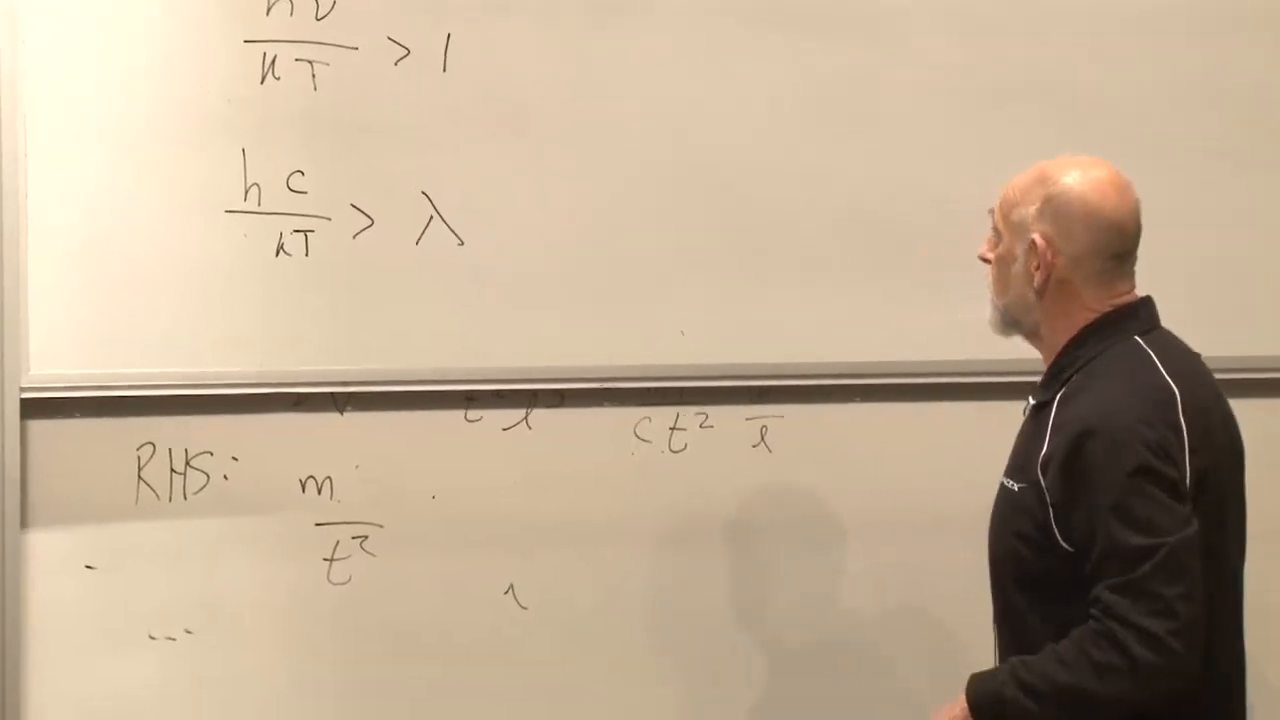
\includegraphics[width=0.82\textwidth]{lecture_07_figure_02.png}\caption{칠판에 적힌 열적 전환. 위쪽에서 잘려 보이는 식은 \(h\nu/(kT)>1\)이고, 아래쪽에서 선명하게 보이는 식은 \(hc/(kT)>\lambda\)이다. 아래쪽 칠판에 희미하게 남은 흔적은 식의 근거로 사용하지 않았다.}\label{fig:c07-thermal-board}\lectureframe{00:44:42.840}\end{figure}

\(\nu=c/\lambda\)을 사용하면 전환 조건에서 대략적인 열적 파장을 정의할 수 있다.
\begin{equation}
\boxed{\lambda_{\rm th}\sim\frac{hc}{k_BT}}.
\label{eq:c07-thermal-wavelength}
\end{equation}
이보다 짧은 파장은 지수적으로 억제된 꼬리 영역에 놓인다. 스펙트럼을 진동수 단위로 그리는지 파장 단위로 그리는지에 따라 달라지는 수치 계수를 제외하면, 복사 에너지의 대부분은 이 정도 파장의 광자가 운반한다.

\begin{classroomqa}
\audiencequestion{플랑크는 여기서 사용하는 전자--양성자 플라스마 모형으로부터 스펙트럼을 얻었나요?}
\lecturerresponse{아니다. 그는 경험적인 스펙트럼 정보와 파장 정점이 온도에 반비례한다는 사실을 이미 보여 준 빈의 변위 법칙을 결합했다. 이 비례 관계에서 새로운 상수 \(h\)가 드러났다. 플랑크는 그 결과를 물질 벽의 진동자와 연결했으며, 복사장의 완전한 양자 해석은 나중에 나왔다. \lecturetimestamp{00:37:06--00:39:25}}\end{classroomqa}

\begin{classroomqa}
\audiencequestion{차원 검산에서 왜 \(c\)의 거듭제곱 하나를 놓친 것처럼 보였나요?}
\lecturerresponse{처음에 강도라고 부른 양은 부피 단위와 진동수 단위 구간당 에너지로 정의되었지만, \(2h\nu^3/c^2\)가 포함된 익숙한 식은 면적과 입체각 단위 구간당 스펙트럼 복사휘도다. 스펙트럼 에너지 밀도에는 \(c^{-3}\)와 각도 인자가 들어가며, 이는 식~\eqref{eq:c07-planck}에 나타나 있다. 이 수정은 정규화 관례를 바꾸지만, 무차원 비 \(h\nu/(k_BT)\)나 열적 파장을 바꾸지는 않는다. \lecturetimestamp{00:39:33--00:44:51}}\end{classroomqa}

정규화를 제외하면 플랑크 스펙트럼은 보편적인 형태를 가진다. 식~\eqref{eq:c07-planck}은 다음과 같이 쓸 수 있다.
\begin{equation}
u_\nu(T)=T^3\,F\!\left(\frac{\nu}{T}\right),
\label{eq:c07-scaling-form}
\end{equation}
상수들은 \(F\)에 흡수했다. \(T\)를 높이면 진동수 축과 전체 높이가 함께 재조정되며, 같은 무차원 곡선이 다시 나타난다. 파장으로 보면 온도가 높아질수록 스펙트럼이 더 짧은 파장 쪽으로 압축된다.

\begin{figure}[htbp]\centering
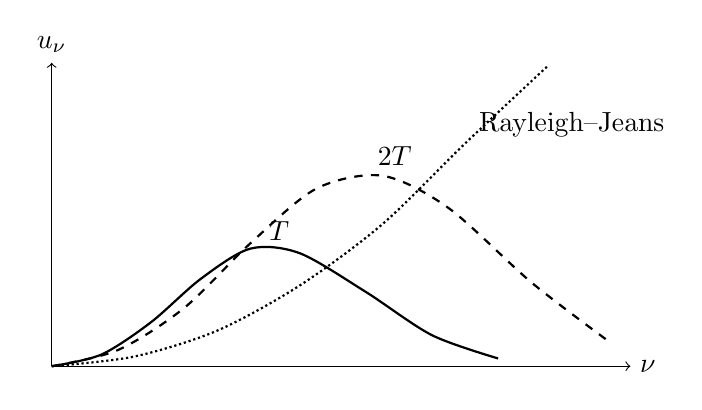
\begin{tikzpicture}[x=1.05cm,y=0.82cm]
\draw[->] (0,0)--(7.0,0) node[right] {\(\nu\)};
\draw[->] (0,0)--(0,4.7) node[above] {\(u_\nu\)};
\draw[densely dotted,thick] plot[smooth] coordinates
  {(0,0) (1,0.15) (2,0.55) (3,1.25) (4,2.20) (5,3.45) (6,4.65)};
\draw[thick] plot[smooth] coordinates
  {(0,0) (0.6,0.18) (1.2,0.68) (1.8,1.35) (2.4,1.82) (3.0,1.75) (3.8,1.15) (4.6,0.48) (5.4,0.12)};
\draw[thick,dashed] plot[smooth] coordinates
  {(0,0) (0.8,0.25) (1.6,0.90) (2.4,1.90) (3.2,2.75) (4.0,2.95) (4.8,2.45) (5.8,1.30) (6.7,0.42)};
\node[anchor=west] at (5.05,3.75) {Rayleigh--Jeans};
\node at (2.75,2.10) {\(T\)};
\node at (4.15,3.25) {\(2T\)};
\end{tikzpicture}\caption{고전 스펙트럼은 제한 없이 증가하지만 플랑크 스펙트럼은 정점을 지나 꺾인다. 온도를 높이면 특성 진동수가 커지고 무차원 형태는 유지된다.}\label{fig:c07-planck-redraw}\end{figure}

현재 우주에 있는 광자의 압도적 다수는 마이크로파 배경에 속하며, 특성 파장은 밀리미터 정도다. 식~\eqref{eq:c07-thermal-wavelength}은 이 파장을 수 켈빈과 연결하며, 여기서는 관례에 따라 \(3\,\mathrm{K}\)로 반올림한다. 파장만으로는 대략적인 대응 관계만 알 수 있다. 더 강한 증거는 여러 진동수에서 측정한 결과가 완전한 흑체 곡선과 매우 높은 정밀도로 일치한다는 점이다.

\begin{classroomqa}
\audiencequestion{마이크로파 배경 광자 하나는 어느 정도 공간을 차지하나요?}
\lecturerresponse{광자에는 보편적이고 경계가 뚜렷한 크기가 없다. 공간적 퍼짐이 상태에 따라 달라지는 파동 묶음으로 준비할 수 있으며, 파장은 진동의 척도를 정한다. 열적 배경에서는 특성 파장과 자연스러운 파동 묶음의 척도 모두 밀리미터 정도지만, 어느 쪽도 작은 고전적 물체의 반지름으로 여겨서는 안 된다. \lecturetimestamp{00:57:16--00:59:05}}\end{classroomqa}

\section{팽창은 흑체 형태를 보존한다}

먼저 이온화된 수소와 복사가 평형을 이루는 뜨거운 상자에서 시작하자. 상자가 팽창하면 내용물이 일을 하고 에너지 밀도가 낮아지며 온도도 내려간다. 결국 전자와 양성자는 중성 원자로 결합한 상태를 유지한다. 원자가 형성되는 과정을 \emph{재결합}이라 하고, 광자--물질 산란의 효율이 떨어지는 과정을 \emph{분리}라 한다. 두 과정은 밀접하게 연관되어 있지만, 서로 다른 물리적 사건을 가리킨다.

분리 뒤에는 물질과 복사가 더 이상 공통 온도를 공유하지 않는다. 그래도 광자 스펙트럼은 플랑크 형태를 유지한다. 자유롭게 전파되는 모든 파장은 같은 팽창 인자만큼 늘어난다.
\begin{equation}
\lambda\propto a,
\qquad
\nu\propto a^{-1}.
\end{equation}
플랑크 곡선은 \(\nu/T\)에 따라 달라지므로, 이렇게 균일한 적색편이를 주면 복사에 다음 온도를 부여하는 것과 같다.
\begin{equation}
\boxed{T_\gamma\propto a^{-1}.}
\label{eq:c07-temperature-scaling}
\end{equation}
따라서 팽창은 충돌이 계속 스펙트럼을 다시 만들어 주지 않아도 그 형태를 보존한다. 물질은 이후에 독자적인 열적 역사를 따른다.

그러므로 관측된 마이크로파 배경은 평형 분포의 화석이다. 자유 전하가 효율적으로 산란하던 시기에 흑체 형태가 형성되었고, 이후 균일한 우주론적 적색편이에 실려 현재까지 전해졌다. 별빛, 감마선 및 그 밖의 후기 천체 기원 복사도 존재하지만, 그 수는 잔존 광자 집단에 비해 적으며 천체물리학적 기원도 식별할 수 있다.

\begin{classroomqa}
\audiencequestion{복사가 물질과 더 이상 평형을 이루지 않는데도 어떻게 흑체 형태를 유지할 수 있나요?}
\lecturerresponse{평형 스펙트럼을 만드는 데는 충돌이 필요하지만, 완벽하게 균일한 팽창 아래에서 그 스펙트럼을 보존하는 데는 충돌이 필요하지 않다. 모든 파장을 같은 인자로 늘리면 한 플랑크 스펙트럼이 더 낮은 온도의 다른 플랑크 스펙트럼으로 바뀐다. 광자는 물질과 온도를 공유하지 않게 되지만, 광자 자체의 흑체 온도는 유지한다.}\end{classroomqa}

\section{재결합은 왜 그렇게 늦게 일어나는가}

오늘날의 파장과 분리 시기의 파장은 다음 관계를 따른다.
\begin{equation}
\frac{\lambda_0}{\lambda_{\rm dec}}
=
\frac{a_0}{a_{\rm dec}}
=
\frac{T_{\rm dec}}{T_0}.
\label{eq:c07-decoupling-ratio}
\end{equation}
분리가 수학적으로 순간에 일어나는 것은 아니지만, 이후 역사에 비하면 충분히 짧은 기간에 이루어지므로 특성 스케일 인자와 온도를 부여할 수 있다. 여기서 \(T_0\)는 은하간 물질의 운동 온도가 아니라 CMB 온도를 뜻한다.

수소 바닥 상태의 이온화 에너지는 다음과 같다.
\begin{equation}
\chi_H=13.6\,\mathrm{eV}.
\end{equation}
첫 추측으로는 \(k_BT\sim\chi_H\)로 두어, 특성 광자가 원자를 이온화할 수 있게 하면 된다. 그러나 열 스펙트럼에는 고에너지 꼬리가 있고 우주에는 광자가 엄청나게 많으므로, 이 추정은 실제보다 훨씬 높은 온도를 준다.

\begin{figure}[htbp]\centering
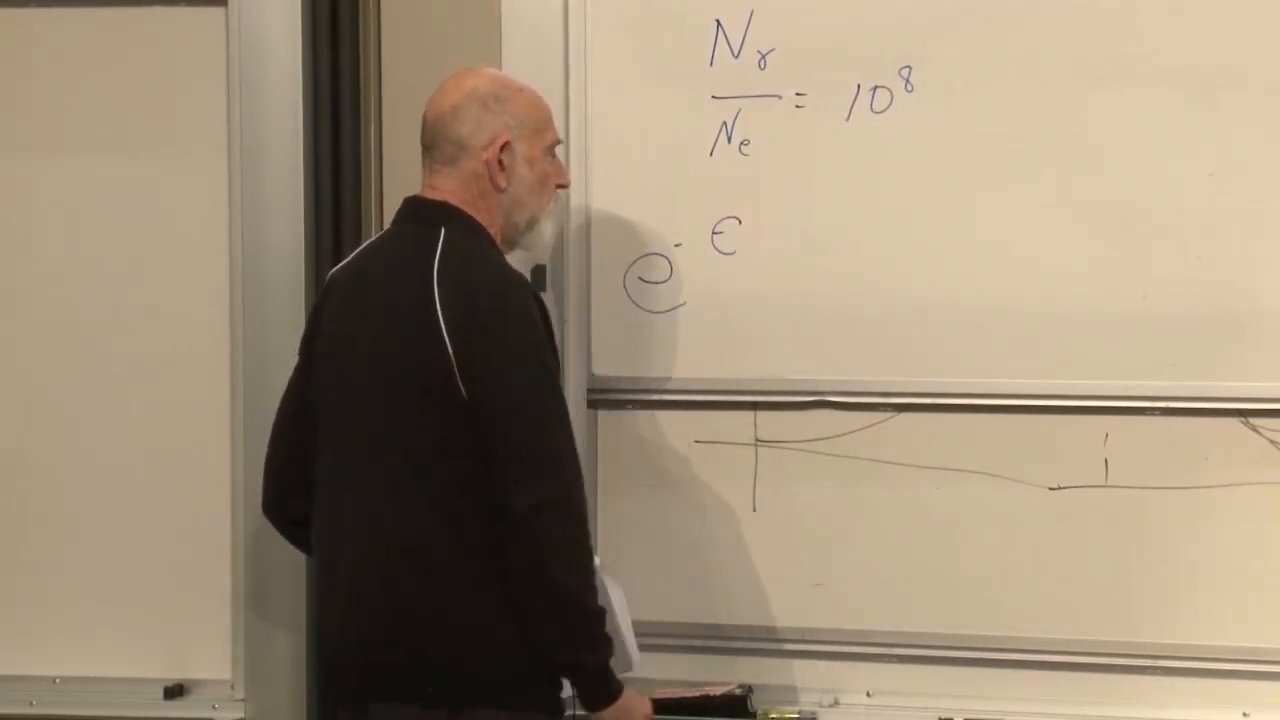
\includegraphics[width=0.82\textwidth]{lecture_07_figure_03.png}\caption{칠판에 관측된 존재비 \(N_\gamma/N_e=10^8\)와 광자 에너지 기호 \(\epsilon\)가 나온다. 지수항의 시작 부분만 보이며, 완성된 볼츠만 인자는 말로 이어지는 유도 과정에서 나온다.}\label{fig:c07-boltzmann-board}\lectureframe{01:06:10.631}\end{figure}

여기서 사용하는 반올림한 존재비는 다음과 같다.
\begin{equation}
\frac{N_\gamma}{N_e}\sim10^8.
\label{eq:c07-photon-electron-ratio}
\end{equation}
이 값은 측정된 CMB 광자 밀도와 보통 물질의 양을 비교해 추론한다. 광자 에너지가 \(\epsilon\)일 때 고에너지 꼬리는 볼츠만 형태를 따른다.
\begin{equation}
P(\epsilon)\propto e^{-\epsilon/(k_BT)}.
\end{equation}
따라서 원자 하나당 이용할 수 있는 이온화 광자 수는 다음과 같이 추산한다.
\begin{equation}
10^8 e^{-\chi_H/(k_BT)}.
\end{equation}
이 양이 대략 1까지 떨어질 때까지 이온화가 유효하게 유지된다.

로그를 취하면 다음을 얻는다.
\begin{equation}
\frac{\chi_H}{k_BT}
\sim
\ln 10^8
\simeq18.4,
\end{equation}
또는 목표로 한 정확도에서는,
\begin{equation}
k_BT\sim\frac{\chi_H}{20}.
\label{eq:c07-tail-estimate}
\end{equation}
꼬리에 있는 이온화 광자 하나가 원자 하나를 이온화하기에 충분하므로, 특성 광자 에너지는 문턱 에너지보다 훨씬 낮아도 된다.

\begin{classroomqa}
\audiencequestion{꼬리 추정은 문턱에 정확히 해당하는 광자만 세나요, 아니면 그보다 높은 에너지의 광자를 모두 세나요?}
\lecturerresponse{문턱 에너지 이상인 광자를 모두 센다. 꼬리는 지수적으로 감소하므로 그 적분값의 대부분은 \(\chi_H\)에 가까운 에너지에서 나온다. 따라서 단순한 지수 추정으로도 관련된 규모를 포착할 수 있다. \lecturetimestamp{01:08:39--01:08:54}}\end{classroomqa}

\begin{classroomqa}
\audiencequestion{비 \(N_\gamma/N_e\)도 분리 시기에 대략 \(10^8\)였나요?}
\lecturerresponse{여기서 사용한 근사에서는 그렇다. 분리 시기부터 온도가 훨씬 더 높았던 시기까지는 팽창이 두 집단을 같은 부피 인자만큼 희석하며, 어느 한쪽의 비율을 바꿀 만큼 두 종을 생성하거나 파괴하지 않는다. 더 높은 온도에서는 쌍 생성 반응을 고려하도록 장부를 새로 맞춰야 한다. \lecturetimestamp{01:08:54--01:09:57}}\end{classroomqa}

\begin{classroomqa}
\audiencequestion{별에서 방출된 광자도 이 계산에 유의미하게 기여하나요?}
\lecturerresponse{아니다. 재결합 시기에는 별이 아직 존재하지 않았고, 오늘날에도 별빛 광자는 CMB 광자 집단에서 차지하는 비율이 아주 작다. 식~\eqref{eq:c07-photon-electron-ratio}의 비는 잔존 열적 광자를 가리킨다. \lecturetimestamp{01:11:44--01:12:39}}\end{classroomqa}

\begin{classroomqa}
\audiencequestion{전자가 양성자와 재결합할 때 방출된 광자가 흑체 스펙트럼에 뚜렷한 수소 특징을 남기지 않나요?}
\lecturerresponse{산란과 흡수가 팽창보다 빠르게 일어나는 동안 복사는 계속 재처리되어 열평형에 가까운 상태를 유지한다. 동결이 충분히 급격했다면 왜곡이 남을 수 있지만, 평형에 가까운 상태에서 재결합이 느리게 진행되므로 큰 고립 선이 흑체 형태를 대체하지는 않는다. \lecturetimestamp{01:12:42--01:14:07}}\end{classroomqa}

그 결과 얻는 교실 수준의 추정값은 \(T_{\rm dec}\sim4\times10^3\,\mathrm{K}\)이다. \(\chi_H/20\)를 직접 환산하면 다소 더 높은 값이 나오므로, 유효 분모가 \(40\)에 더 가까울 수 있다는 제안이 나온다. 이는 모순이 아니라, 전체 이온화 균형을 꼬리 광자 수 하나로 대체한 접근이 얼마나 거친지를 보여 준다. 제어된 평형 분석에는 사하 관계식을 사용한다.
\begin{equation}
\frac{x_e^2}{1-x_e}
=
\frac{1}{n_H}
\left(\frac{m_e k_BT}{2\pi\hbar^2}\right)^{3/2}
e^{-\chi_H/(k_BT)},
\label{eq:c07-saha}
\end{equation}
그다음에는 비평형 재결합 동역학을 고려한다. 이 거친 논증의 가치는 지배적인 물리를 짚어 준다는 데 있다. 바리온 대 광자 비가 매우 작기 때문에 중성 원자가 살아남는 온도는 \(\chi_H/k_B\)보다 훨씬 낮아진다.

\section{최종 산란면까지의 적색편이}

\(T_0\simeq3\,\mathrm{K}\)와 \(T_{\rm dec}\sim4\times10^3\,\mathrm{K}\)을 사용해 식~\eqref{eq:c07-decoupling-ratio}에 대입하면 다음을 얻는다.
\begin{equation}
\boxed{
\frac{a_0}{a_{\rm dec}}
\sim
\frac{T_{\rm dec}}{T_0}
\sim10^3
}.
\label{eq:c07-decoupling-expansion}
\end{equation}
이를 다시 쓰면 최종 산란 적색편이는 대략 \(10^3\)이다. 이 시기 전에는 이온화된 플라스마가 불투명했고, 이후에는 광자가 거의 자유롭게 전파되었다.

이 열적 사건은 뜨거운 팽창이 시작된 뒤 불과 수십만 년 후에 일어났다. 이 대화에서는 관례적으로 대략 \(380{,}000\)년으로 제시한다. 이 기간은 이후의 우주 나이에 비하면 매우 짧다. 분리 뒤 길이는 약 \(10^3\)배, 공변 부피 요소는 약 \(10^9\)배 커졌다.

분리는 열적 이정표 가운데 하나일 뿐, 그 사이 역사에서 일어난 유일한 사건은 아니다. 은하 형성, 별 형성, 블랙홀 형성은 모두 그 뒤에 일어나지만, 열적 이정표를 명확히 따라가기 위해 여기서는 다루지 않는다.

멀리 내다보는 일은 과거를 보는 일이다. 가까운 구각은 최근 시기를, 더 먼 구각은 더 이른 시기를 보여 준다. 우리의 과거 빛원뿔은 결국 재결합 시기와 만나며, 그 시기와 교차하는 면이 최종 산란면이다. 그보다 이른 전자기 복사는 자유 전하에 반복해서 산란했으므로 우리에게 직접 도달할 수 없었다.

\begin{figure}[htbp]\centering
\begin{coursefitfigure}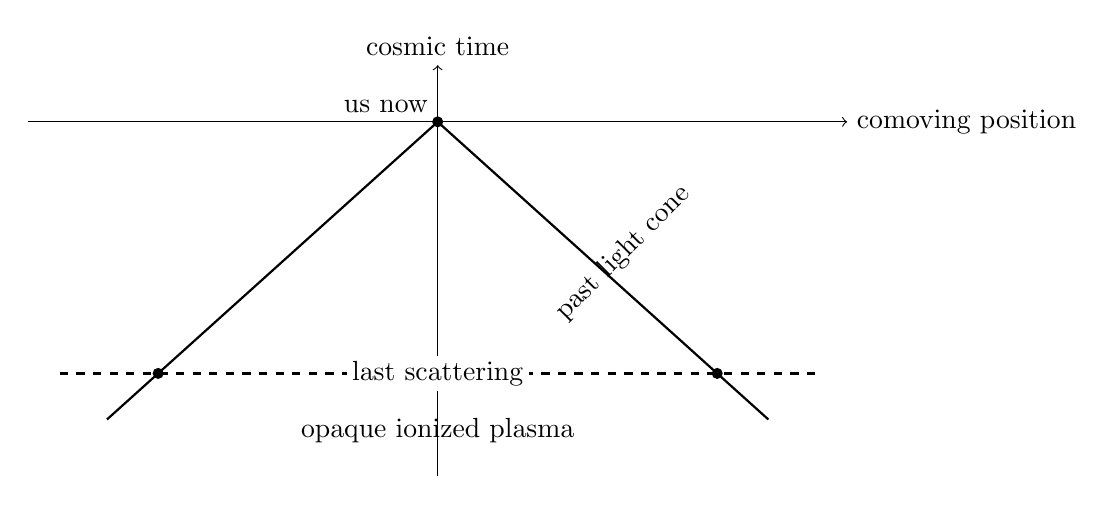
\begin{tikzpicture}[x=1.0cm,y=0.9cm]
\draw[->] (0,0)--(0,5.8) node[above] {cosmic time};
\draw[->] (-5.2,5.0)--(5.2,5.0) node[right] {comoving position};
\draw[thick] (0,5.0)--(-4.2,0.8);
\draw[thick] (0,5.0)--(4.2,0.8);
\draw[thick,dashed] (-4.8,1.45)--(4.8,1.45);
\fill (0,5.0) circle (2pt) node[above left] {us now};
\fill (-3.55,1.45) circle (2pt);
\fill (3.55,1.45) circle (2pt);
\node[fill=white,inner sep=2pt] at (0,1.45) {last scattering};
\node at (0,0.65) {opaque ionized plasma};
\node[rotate=45] at (2.35,3.15) {past light cone};
\end{tikzpicture}\end{coursefitfigure}\caption{전자기 관측으로 과거 빛원뿔을 따라 되짚을 수 있는 범위는 최종 산란면까지다. 그 이전의 광자는 이온화된 플라스마에서 반복적으로 산란했다.}\label{fig:c07-last-scattering}\end{figure}

\begin{classroomqa}
\audiencequestion{분리가 일어나면 더 이른 시대를 관측할 수 있는 모든 방법이 사라지나요?}
\lecturerresponse{플라스마가 광자에 불투명했으므로 분리는 전자기파를 이용한 직접 관측을 끝낸다. 더 약하게 상호작용하는 메신저는 그보다 이른 시기에 탈출할 수 있다. 원시 중성미자는 원리적으로 더 깊은 층을 탐사할 수 있고, 중력 복사는 그보다 더 이른 시기의 정보를 전달할 수 있다. 따라서 최종 산란보다 이전 시기에 대한 지식은 상당 부분 간접적이지만 임의적인 것은 아니다. \lecturetimestamp{01:32:27--01:36:31}}\end{classroomqa}

\begin{classroomqa}
\audiencequestion{시작 시점의 \(a\)는 얼마였으며, 우주는 반드시 작고 유한한 천체였나요?}
\lecturerresponse{평탄한 공간에서는 스케일 인자 \(a\)의 정규화가 임의적이므로, 스케일 인자들의 비만 불변적인 의미를 갖는다. 음의 곡률을 가진 공간 단면도 무한할 수 있다. 닫힌 \(k=+1\) 우주에는 유한한 곡률 반경이 있지만, 관측으로 정해지는 것은 여전히 팽창 비율이지, 알려진 원시 크기가 아니다. 뜨거운 빅뱅이라는 말 자체가 모든 공간이 작은 공이었다는 뜻은 아니다. \lecturetimestamp{01:30:05--01:32:22}}\end{classroomqa}

\begin{classroomqa}
\audiencequestion{CMB는 은하보다 오래되었는데, CMB를 보면 관측 가능한 영역 너머에도 오늘날 은하가 있는지 알 수 있나요?}
\lecturerresponse{아니다. CMB는 먼 영역의 현재 모습을 보여 주는 것이 아니라 분리 시기의 모습을 보여 준다. 충분히 먼 곳의 현재 은하에서 나온 빛은 우리에게 도달할 시간이 없었다. 지평선 너머에도 은하 집단이 계속 존재할 것이라고 보는 근거는 CMB가 직접 보여 주는 모습이 아니라 관측된 대규모 균질성과 눈에 보이는 경계가 없다는 사실이다. \lecturetimestamp{01:59:01--02:00:58}}\end{classroomqa}

따라서 현재부터 은하 형성과 분리를 거쳐 물질--복사 동등 시기까지 거슬러 올라가는 연대표를 얻는다. 그보다 더 이른 시기에는 작아지는 스케일 인자에 따라 온도가 높아지고 새로운 입자 종이 나타난다.

\section{물질--복사 동등 시기}

분리 시기보다 더 과거로 가면 또 다른 이정표가 나타난다. 비상대론적 물질과 복사는 서로 다른 방식으로 희석된다.
\begin{equation}
\rho_m\propto a^{-3},
\qquad
\rho_r\propto a^{-4},
\qquad
\frac{\rho_m}{\rho_r}\propto a.
\label{eq:c07-equality-scaling}
\end{equation}
후기 우주에서는 물질이 우세하지만, 충분히 작은 \(a\)에서는 복사가 필연적으로 우세해진다. 이에 따라 팽창 법칙도 물질 지배기 거동인 \(a\propto t^{2/3}\)에서 복사 지배기 거동인 \(a\propto t^{1/2}\)으로 바뀐다.

일부러 거칠게 잡은 추정은 광자 수 \(10^8\)개 대 양성자 하나, CMB 광자의 특성 에너지 \(10^{-4}\,\mathrm{eV}\), 양성자 정지 에너지 \(10^9\,\mathrm{eV}\)에서 시작한다. 암흑물질을 무시하면 다음을 얻는다.
\begin{equation}
\left(\frac{\rho_m}{\rho_r}\right)_0
\sim
\frac{10^9}{10^8\,10^{-4}}
\sim10^5.
\end{equation}
그러나 이 논증을 보정해야 한다. 암흑물질의 질량은 발광 바리온보다 상당히 크므로, 반올림한 추정값은 \(10^6\)으로 올라간다. 이 산술을 따르면 식~\eqref{eq:c07-equality-scaling}은 동등 시기를 다음과 같이 정한다.
\begin{equation}
\frac{a_{\rm eq}}{a_0}\sim10^{-6},
\qquad
\frac{T_{\rm eq}}{T_0}\sim10^6.
\label{eq:c07-equality-estimate}
\end{equation}
이는 척도를 정하기 위한 교실 수준의 추정값이지, 정밀한 우주론 매개변수 적합 결과가 아니다. 이 추정의 목적은 서로 다른 \(a\) 거듭제곱이 연속되는 열적 시대들의 위치를 어떻게 정하는지 보여 주는 것이다.

복사 지배 시대는 전자기적 최종 산란 장벽 너머에 있지만, 그 존재는 후기 우주에서 측정된 밀도와 알려진 스케일링 법칙으로부터 따라 나온다. 온도를 더 높여 가면, 양성자·전자·광자의 수가 각각 고정되어 있다는 가정은 결국 성립하지 않는다. 에너지가 큰 충돌이 질량이 있는 입자--반입자 쌍을 만들기 시작하기 때문이다.

\begin{classroomqa}
\audiencequestion{광자 수와 양성자 수가 보존된다는 말에는 별빛과 임의로 높은 온도까지 포함되나요?}
\lecturerresponse{아니다. 이 말은 입자 수를 바꾸는 반응이 효과적이지 않은 기간 동안의 잔존 CMB 집단에 적용된다. 별빛은 나중에 생겼고 광자 수에서 차지하는 비율도 무시할 만하다. 온도가 충분히 높아지면 쌍 생성으로 입자 구성이 달라져 각 입자 종의 수가 따로 보존되지 않는다. 재결합으로 추가되는 광자는 기껏해야 전자 하나당 대략 한 개이며, 기존 CMB 광자 수의 \(10^8\)분의 1에 불과하다. \lecturetimestamp{01:26:24--01:27:40}}\end{classroomqa}

\section{쌍 생성과 거의 대칭인 수프}

온도가 대략
\begin{equation}
T\sim10^{10}\,\mathrm{K},
\qquad
\frac{a_0}{a}\sim10^{14},
\end{equation}
일 때 특성 광자 에너지는 메가전자볼트 정도로, 전자--양전자 쌍을 만드는 데 필요한 정지 에너지 척도와 비슷하다. 그러면 광자 두 개가 다음 반응을 일으킬 수 있다.
\begin{equation}
\gamma+\gamma
\longleftrightarrow
e^-+e^+.
\label{eq:c07-pair-reaction}
\end{equation}
정확한 문턱은 충돌 운동학에 따라 달라지지만, 전자의 정지 에너지 \(m_ec^2\)가 관련 척도를 정한다.

쌍 생성과 소멸은 빠르게 서로 균형을 이룬다. 쌍이 너무 적으면 광자 충돌이 쌍을 보충하고, 너무 많으면 소멸이 그 에너지를 광자로 되돌린다. 따라서 광자, 전자, 양전자의 존재량은 온도에 의해 정해지며, 상대론적 플라스마에서는 모두 비슷한 규모다. 이들은 더 이상 나중에 관측되는 입자 수를 단순하게 기억하지 않는다.

\begin{classroomqa}
\audiencequestion{양성자 전하를 상쇄할 전자가 이미 있는데, 쌍으로 가득 찬 이 플라스마는 어떻게 전기적 중성을 유지하나요?}
\lecturerresponse{각 반응은 음전하와 양전하를 하나씩 만들어 내므로 쌍은 순전하를 더하지 않는다. 쌍은 거의 대칭인 엄청난 입자 집단으로 존재하며, 그 위에 소량의 전자 초과분이 더해져 있다. 개별 전자는 서로 구별할 수 없고, 차이인 \(N_{e^-}-N_{e^+}\)만이 양성자의 전하를 상쇄하는 데 필요한 양을 기억한다. \lecturetimestamp{01:42:31--01:43:14}}\end{classroomqa}

쌍 반응은 합은 바꾸지만 차이는 보존한다.
\begin{equation}
N_{e^-}+N_{e^+}\quad\hbox{changes},
\qquad
N_{e^-}-N_{e^+}=\hbox{constant}.
\label{eq:c07-pair-invariants}
\end{equation}
뜨거운 수프에서는 \(N_{e^-}+N_{e^+}\)가 \(N_\gamma\)와 같은 규모인 반면, 살아남은 초과분은 훨씬 적은 양성자 수와 같은 규모다. 따라서 반올림한 비는 다음과 같다.
\begin{equation}
\boxed{
\frac{N_{e^-}-N_{e^+}}
{N_{e^-}+N_{e^+}}
\sim10^{-8}
}.
\label{eq:c07-asymmetry}
\end{equation}
전자\(10^8\)양전자 쌍 약 --개당 초과 전자가 하나 있었다.

이는 원래의 질문을 뒤집는다. 놀라운 점은 단순히 광자가 많다는 사실이 아니다. 온도가 높을 때 광자와 입자·반입자 쌍은 자연스럽게 비슷한 개수로 존재한다. 문제는 음전하 입자와 양전하 입자의 개수가 왜 서로 다른지, 또 그 상대적 차이가 왜 정확히 영이거나 1 정도의 크기가 아니라 아주 작은지이다. 초기 상태와 쌍 생성이 대칭적이었다면 어느 쪽도 초과하지 않았을 것이다. 이 비영 비대칭의 미시적 기원이 다음 단계 논의에서 다룰 문제다.

온도가 다시 두세 자릿수 규모 더 높아지면 양성자의 내부 구조를 더 이상 무시할 수 없다. 충돌은 쿼크와 반쿼크를 만들고, 양성자는 구성 성분들로 분해된다. 광자, 렙톤, 쿼크, 반쿼크, 글루온 및 충분히 가벼운 암흑 입자가 더 뜨거운 플라스마를 이룬다. 그곳에서는 복사 밀도가 \(a^{-4}\)에 따라 증가하므로 진공 에너지의 동역학적 효과는 무시할 수 있다.

이에 대응하는 쿼크 과잉은 전체 전하 중성 조건에 의해 전자 과잉과 연결된다. 원자가 쿼크 세 개가 바리온 하나를 이루므로 장부를 맞출 때 관례적인 계수 차이가 있지만, 살아남은 바리온 물질과 살아남은 전자는 서로 독립적인 전하 불균형이 아니다. 둘 다 미세한 과잉을 보이는 것은 초기 우주의 잔재다.

전자--양전자 플라스마의 진화를 다시 따라가 보자. 온도가 쌍생성 에너지 척도 아래로 내려가면 역반응은 드물어지는 한편 소멸은 계속된다. 거의 모든 전자는 양전자를 만나고, 쌍의 에너지는 복사로 바뀌며, 서로 짝을 이루지 못한 극소수의 전자만 남는다. 우리 주변의 물질은 한때 엄청나게 많았던 쌍의 대표 표본이 아니라 이 잔여 불균형이다.

\begin{classroomqa}\audiencequestion{전자--양전자 소멸 시기에 양성자는 무엇을 하고 있었나요?}\lecturerresponse{당시 온도는 전자 쌍을 생성하기에는 충분히 높았지만, 양성자--반양성자 쌍을 풍부하게 생성하거나 양성자를 쿼크로 분해하기에는 아직 충분히 높지 않았다. 따라서 양성자 수는 적었지만 계속 유지되었으며, 전하 중성을 위해서는 \(N_{e^-}-N_{e^+}\simeq N_p\)이어야 했다. \lecturetimestamp{01:55:35--01:56:53}}\end{classroomqa}

가시 우주 전체에서 물질 초과의 부호는 같은 것으로 보인다. 강의에서 제시된 관측 근거는 우주선에서 반핵이 발견되지 않는다는 점이다. 이차 충돌로 드물게 반양성자가 생성될 수 있지만, 반은하가 있다면 복잡한 반핵을 내놓을 것으로 예상된다. 이는 강의 당시의 관측에 근거한 논거이지, 관측 가능한 지평선 너머의 영역을 조사했다는 주장은 아니다.

\begin{classroomqa}\audiencequestion{관측된 물질 과잉이 국소적인 요동이고, 우리가 볼 수 있는 범위 너머에는 반물질 영역이 있을 가능성은 없나요?}\lecturerresponse{관측 가능한 엄청나게 넓은 부피 전체에서 부호가 같다는 사실은 무작위 요동으로 설명하기에는 지나치게 일관적이다. 따라서 동역학적 설명이 필요하다. 그러나 관측 가능한 영역 너머에 대해서는 직접적인 증거를 얻을 수 없다. 빛이 우리에게 도달한 범위보다 더 멀리 내다본다는 이유만으로 다른 영역으로 이어지는 가능성을 배제할 수는 없다. \lecturetimestamp{01:56:57--01:58:47}}\end{classroomqa}

\begin{classroomqa}\audiencequestion{물질--반물질 설명은 이미 정밀한 수치 이론인가요? 그리고 이 온도에서 힘의 통일이 일어나나요?}\lecturerresponse{작은 비대칭이 생길 수 있는 과정을 설명하는 정성적 이론은 있지만, 여기서는 반올림한 값 \(10^{-8}\)을 유일한 미시적 모형에서 유도하지 않는다. 힘의 통일은 전자 쌍이 생기던 시기보다 훨씬 높은 온도에서 일어난다. 두 질문 모두 현재 다루는 열적 이정표를 넘어서는 물리학을 필요로 한다. \lecturetimestamp{01:51:36--01:52:24}}\end{classroomqa}

\section{앞으로 기억할 점}

열적 역사는 반응률과 임계값을 기준으로 정리된다. 산란이 빠르면 공통 온도가 형성되고, 중성 원자가 만들어지면 산란체가 사라진다. 그 뒤에는 균일한 팽창으로 동결된 플랑크 스펙트럼이 적색편이하지만 그 형태는 유지된다. 따라서 CMB는 복사의 온도계인 동시에 초기 플라스마에 전자기적으로 직접 접근할 수 있었던 시대의 끝을 나타내는 가시적 표면이다.

광자 과잉 때문에 재결합은 평균 에너지 문제가 아니라 꼬리 분포의 문제가 된다. 비율 \(T_{\rm dec}/T_0\sim10^3\)은 마지막 산란 시기를 가리키며, 물질과 복사의 희석률 차이는 그보다 앞선 등가 시기를 가리킨다. 온도가 더 높아지면 쌍생성으로 전자와 양전자의 전체 수에 관한 기억은 지워지지만, 둘의 미세한 차이는 보존된다. 바리온 부문에도 그대로 나타나는 이 잔여 비대칭은 다음 탐구에서 다루어야 할 설명되지 않은 초기 조건이다.
